%!TEX program = xelatex

\documentclass[10pt]{beamer}

\usepackage[heading=true]{ctex}
% \usepackage[colorlinks,linkcolor=red]{hyperref}

\usepackage{graphicx}
\usepackage{float}
% \usepackage[colorlinks, linkedcolor=red]{hyperref}

% for python
\usepackage{listings}
\usepackage{color}

\definecolor{dkgreen}{rgb}{0,0.6,0}
\definecolor{gray}{rgb}{0.5,0.5,0.5}
\definecolor{mauve}{rgb}{0.58,0,0.82}

\lstset{
    frame=tb,
    language=Python,
    aboveskip=3mm,
    belowskip=3mm,
    showstringspaces=false,
    columns=flexible,
    basicstyle={\small\ttfamily},   
    numbers=none,
    numberstyle=\tiny\color{gray},
    keywordstyle=\color{blue},
    commentstyle=\color{dkgreen},
    stringstyle=\color{mauve},
    breaklines=true,
    breakatwhitespace=true,
    tabsize=3,
}



\usetheme[]{Rochester}

\mode<presentation>

\title{
    \href{https://github.com/Ls-Dai/Cloud-Sever-Tutorial}{云服务器使用说明和相关规定}
}
\author{戴立森}
\date{Nov 12, 2020}

\begin{document}
    \maketitle
    \begin{frame}
        \frametitle{云服务器概况}
            \framesubtitle{云服务器配置、计费}

            {\small
            \begin{table}[h]
                \centering
                \caption{算力对比}\label{tab:tab1}
                    \begin{tabular}{|c|c|c|c|}
                        \hline
                        显卡 & 算力(TFLOPS) & 显存(G) & 相对速度 \\
                        \hline
                        Titan XP(A534) & 10.97 & 12 & 1 \\
                        \hline
                        G4 (RTX2080) & 13.45 & 11 & 1.226 \\
                        \hline
                        Tesla T4 & 8.141 & 16 & 0.742 \\
                        \hline
                        Tesla P40 & 11.76 & 24 & 1.072 \\
                        \hline
                        Tesla P100 & 9.526 & 16 & 0.868 \\
                        \hline
                    \end{tabular}
            \end{table}
            }

    \end{frame}


    \begin{frame}
        \frametitle{云服务器概况}
            \framesubtitle{计费说明}

            {\small
            \begin{table}[h]
                {\centering
                \caption{计费说明}\label{tab:tab1}
                    \begin{tabular}{|p{0.2\columnwidth}|p{0.6\columnwidth}|}
                        \hline
                        项目 & 单位数量单位时间价格 \\
                        \hline
                        1块RTX2080显卡配上8核i5 CPU & 5.84金币/小时 \\
                        \hline
                        存储空间 & 最低80G,需要 0.02金币/小时。超过80G的部分增加量需为50G的倍数,每增加50G需要 0.015金币/小时,四舍五入保留两位小数 \\
                        \hline
                        传输带宽(按带宽计费) & 5M及以下时为每小时0.03金币/Mbps,多出5M的部分需要增加每小时 0.135金币/Mbps \\
                        \hline
                        传输带宽(按流量计费) & 0.78金币/G,带宽大小可自选,上限100Mpbs \\
                        \hline
                    \end{tabular} \\
                }
            \end{table}
            {\tiny \qquad \qquad 注:金币和人民币换算比例为0.92}
            }

    \end{frame}

    \begin{frame}
        \frametitle{开始使用云主机}
            \framesubtitle{演示:创建一个适合使用的云主机}

            % \href{https://ai.blsc.cn/#/support/info}{
            %     
\includegraphics{src/img/Tweet.png}
            %     }
            \centering
            \href{https://ai.blsc.cn/\#/support/info}{
                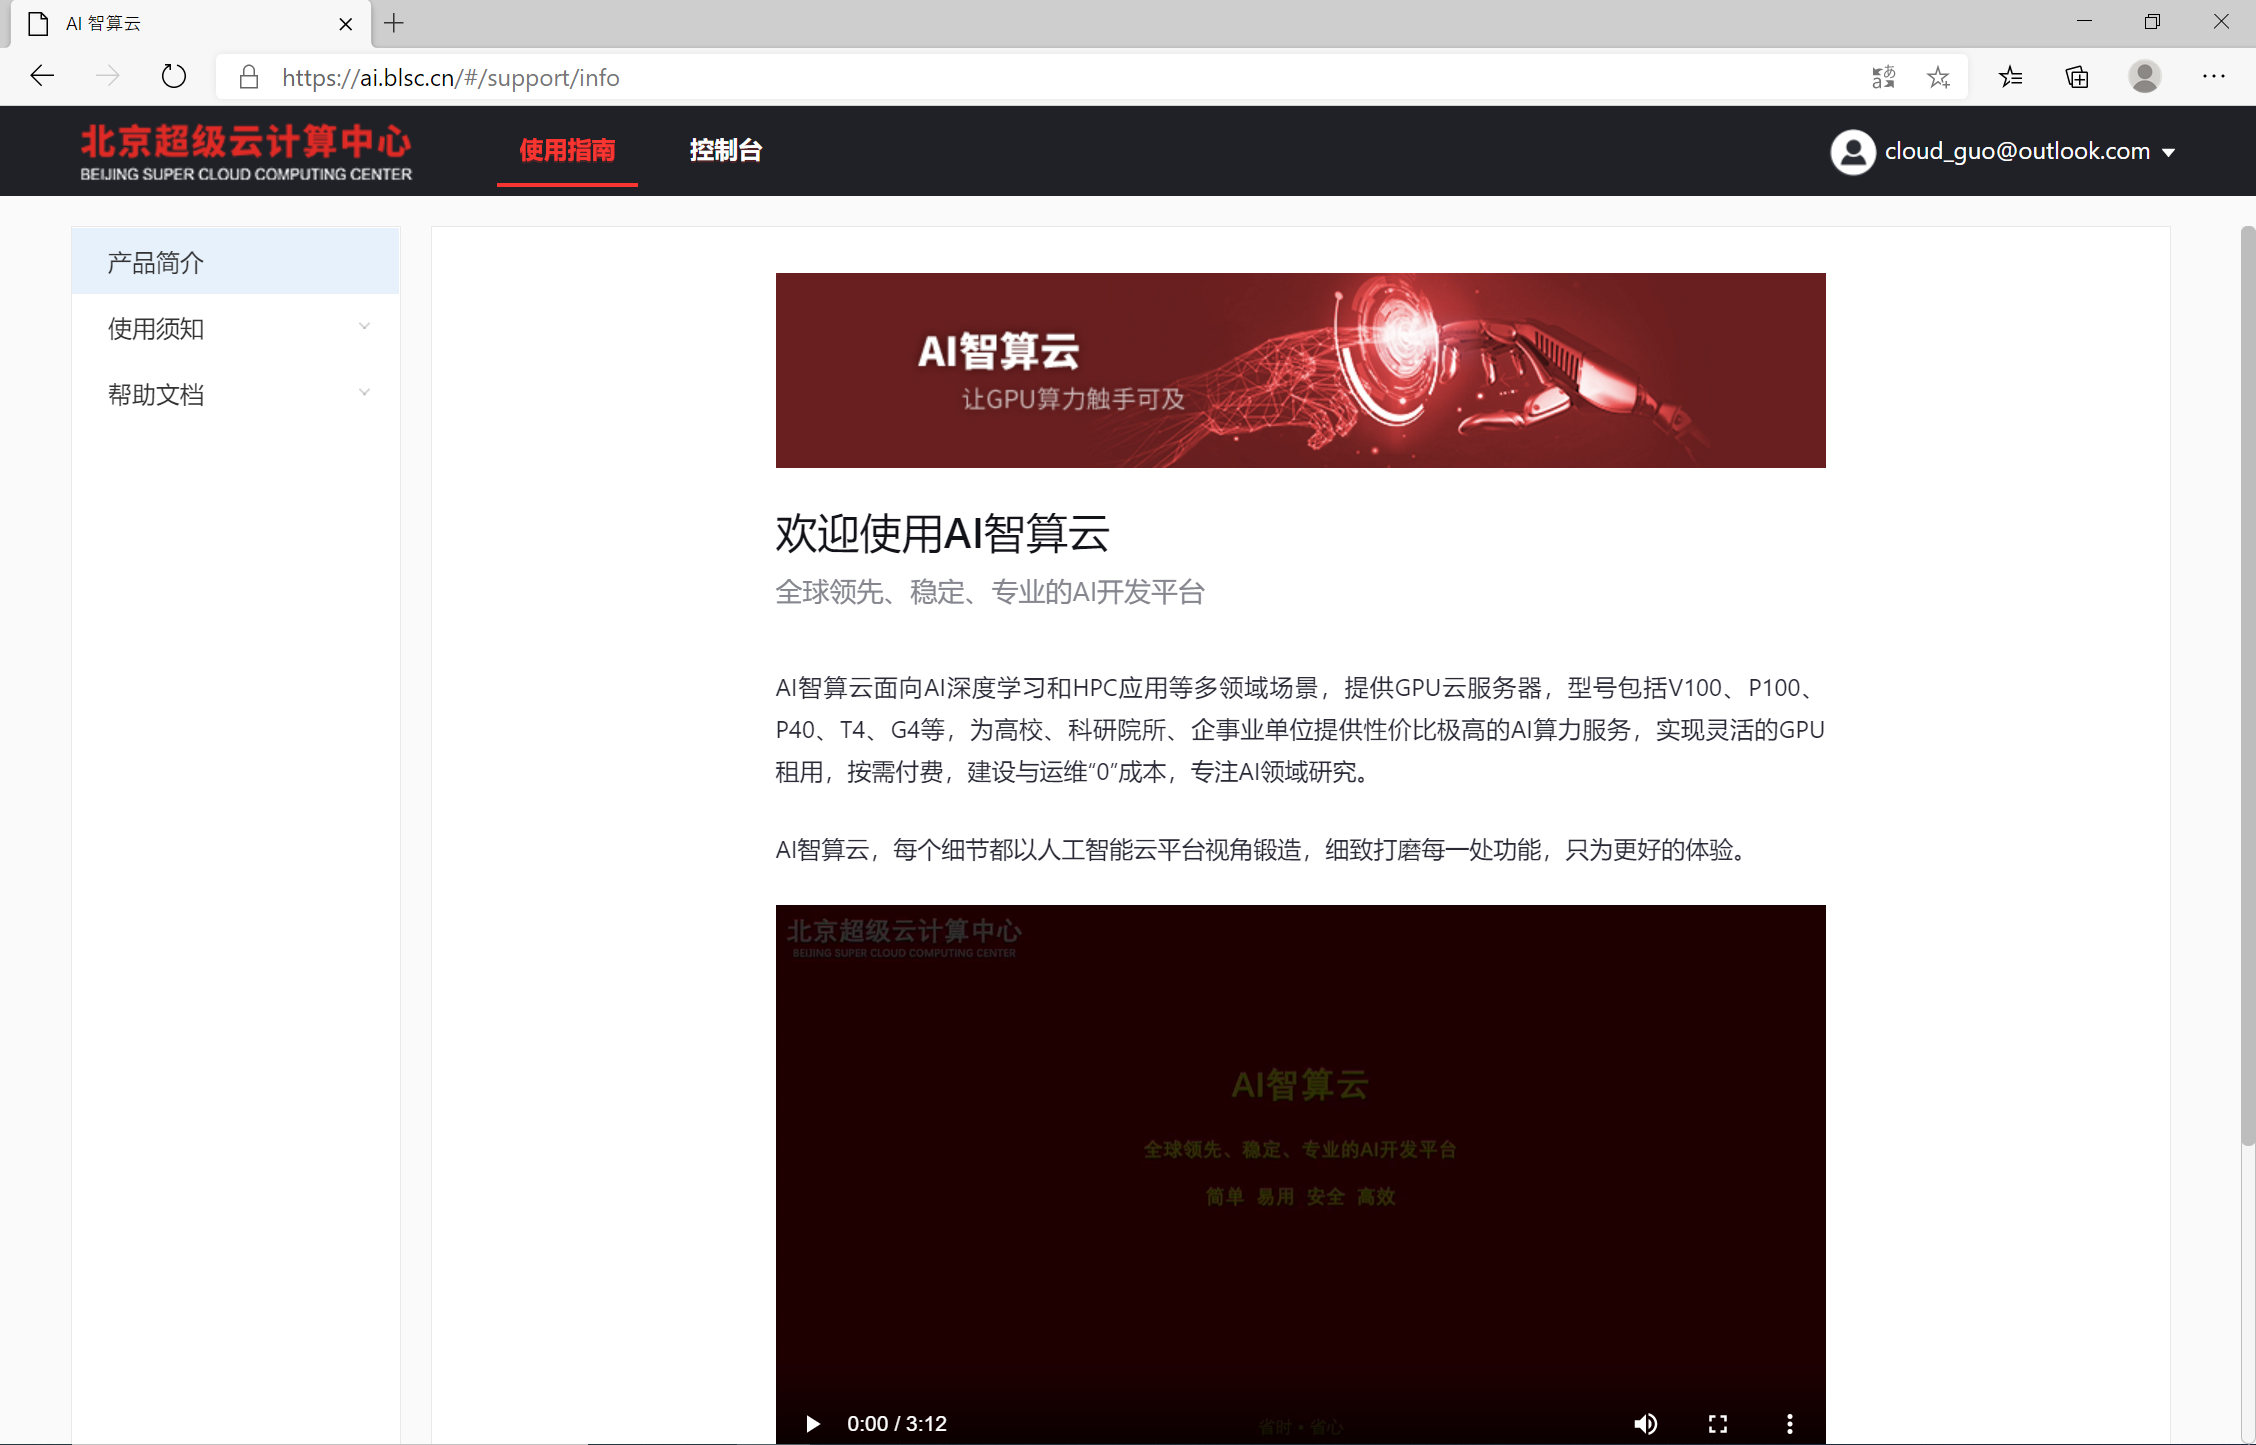
\includegraphics[scale=0.2]{src/img/Welcome.png}
                }

    \end{frame}

    \begin{frame}
        \frametitle{开始使用云主机}
            \framesubtitle{演示:远程交互}

            % \href{https://ai.blsc.cn/#/support/info}{
            %     
\includegraphics{src/img/Tweet.png}
            %     }
            \centering
            \hyperlink{frame5}{
                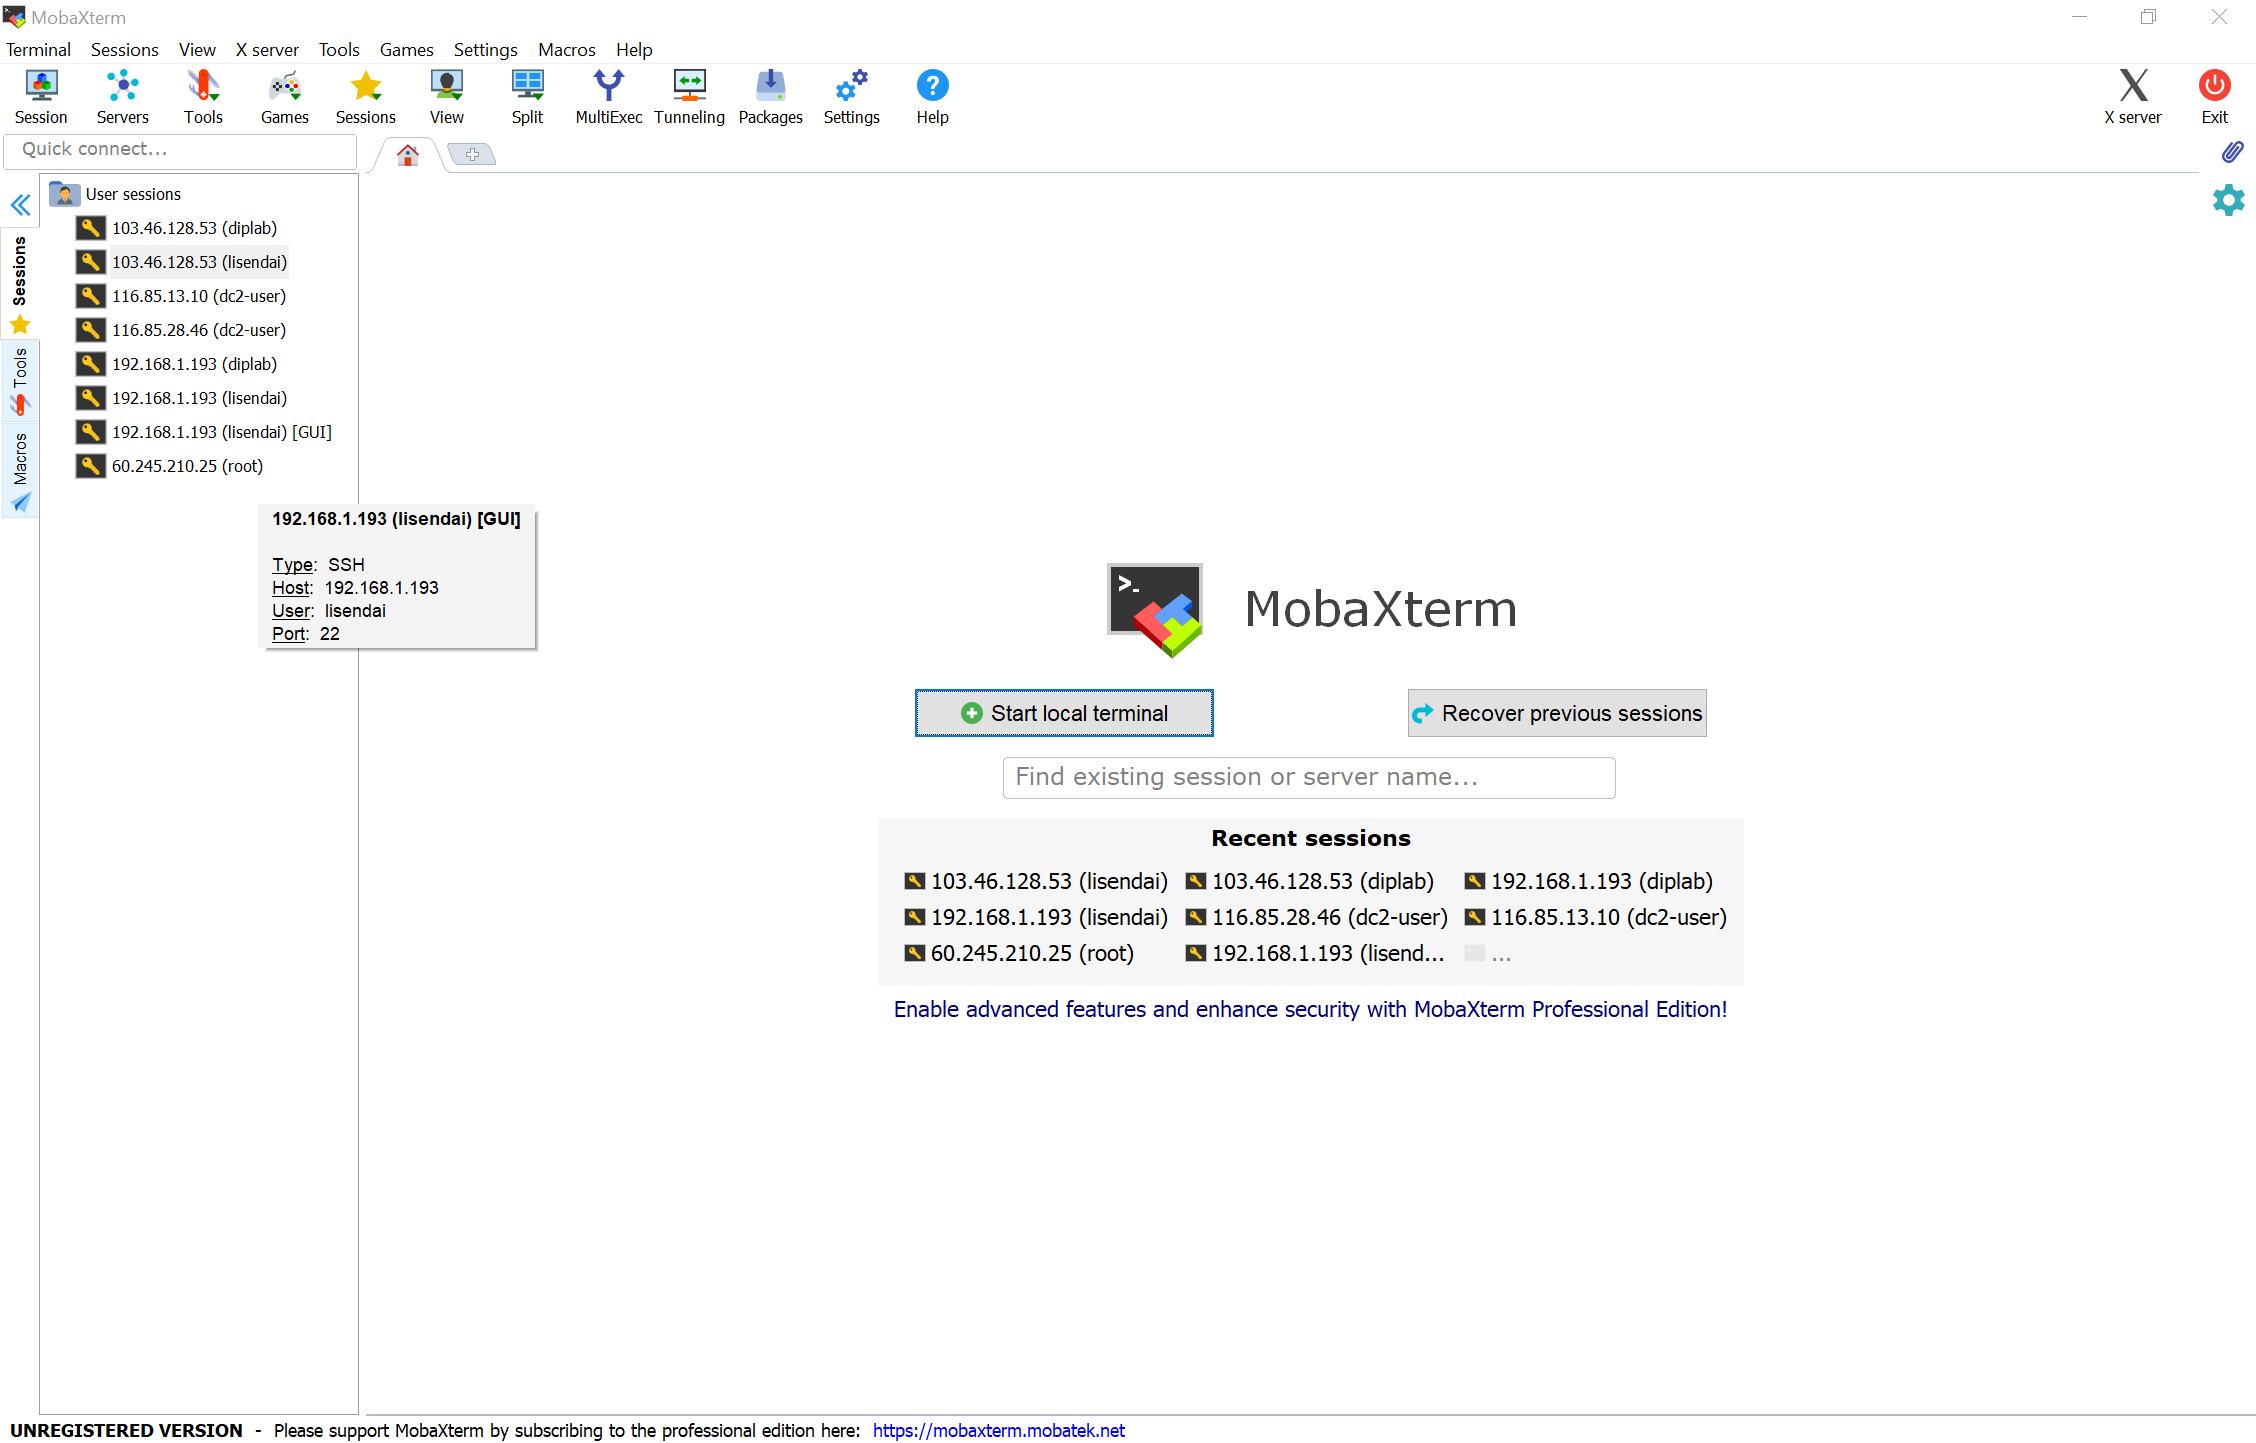
\includegraphics[scale=0.2]{src/img/MobaXterm.png}
                }

    \end{frame}

    \begin{frame}[fragile]
        \frametitle{并行计算(PyTorch)}
            \framesubtitle{基本原理}
                核心代码: \\
                \begin{lstlisting}
torch.nn.DataParallel                    
                \end{lstlisting}
                可将模型发送到多个GPU上进行并行计算,每个GPU都有一个模型的副本。\\
                训练时,每一批 (batch) 的数据会被均匀地分配到所有GPU上进行处理,计算的梯度会被汇总到原始的模型中进行更新。\\
                \hspace*{\fill}
                \begin{itemize}
                    \item 务必保证批的大小(batchsize)大于使用的GPU的数量。
                    \item 在这个训练过程中,因为梯度会被汇总,所以不涉及改变批的大小(batchsize)的问题。
                    \item 因为汇总梯度等原因,GPU(0)一般要被占用更多的显存。
                \end{itemize}

    \end{frame}

    \begin{frame}[fragile]
        \frametitle{并行计算(PyTorch)}
            \framesubtitle{代码讲解}
                % Python code
                \begin{lstlisting}[basicstyle=\small]
import torch.nn as nn
                \end{lstlisting}
                \begin{lstlisting}[basicstyle=\small]
gpus = range(num_gpus)
                \end{lstlisting}
                \begin{lstlisting}[basicstyle=\small]
torch.cuda.device_count
                \end{lstlisting}
                \begin{lstlisting}[basicstyle=\small]
model = nn.DataParallel(model.cuda(), device_ids=gpus, output_device=gpus[0]) 
                \end{lstlisting}

                



    \end{frame}

    \begin{frame}
        \frametitle{云服务器使用规则}
            \framesubtitle{基本信息管理}

            % \href{https://ai.blsc.cn/#/support/info}{
            %     
\includegraphics{src/img/Tweet.png}
            %     }
            \centering
            \href{https://ai.blsc.cn/\#/support/info}{
                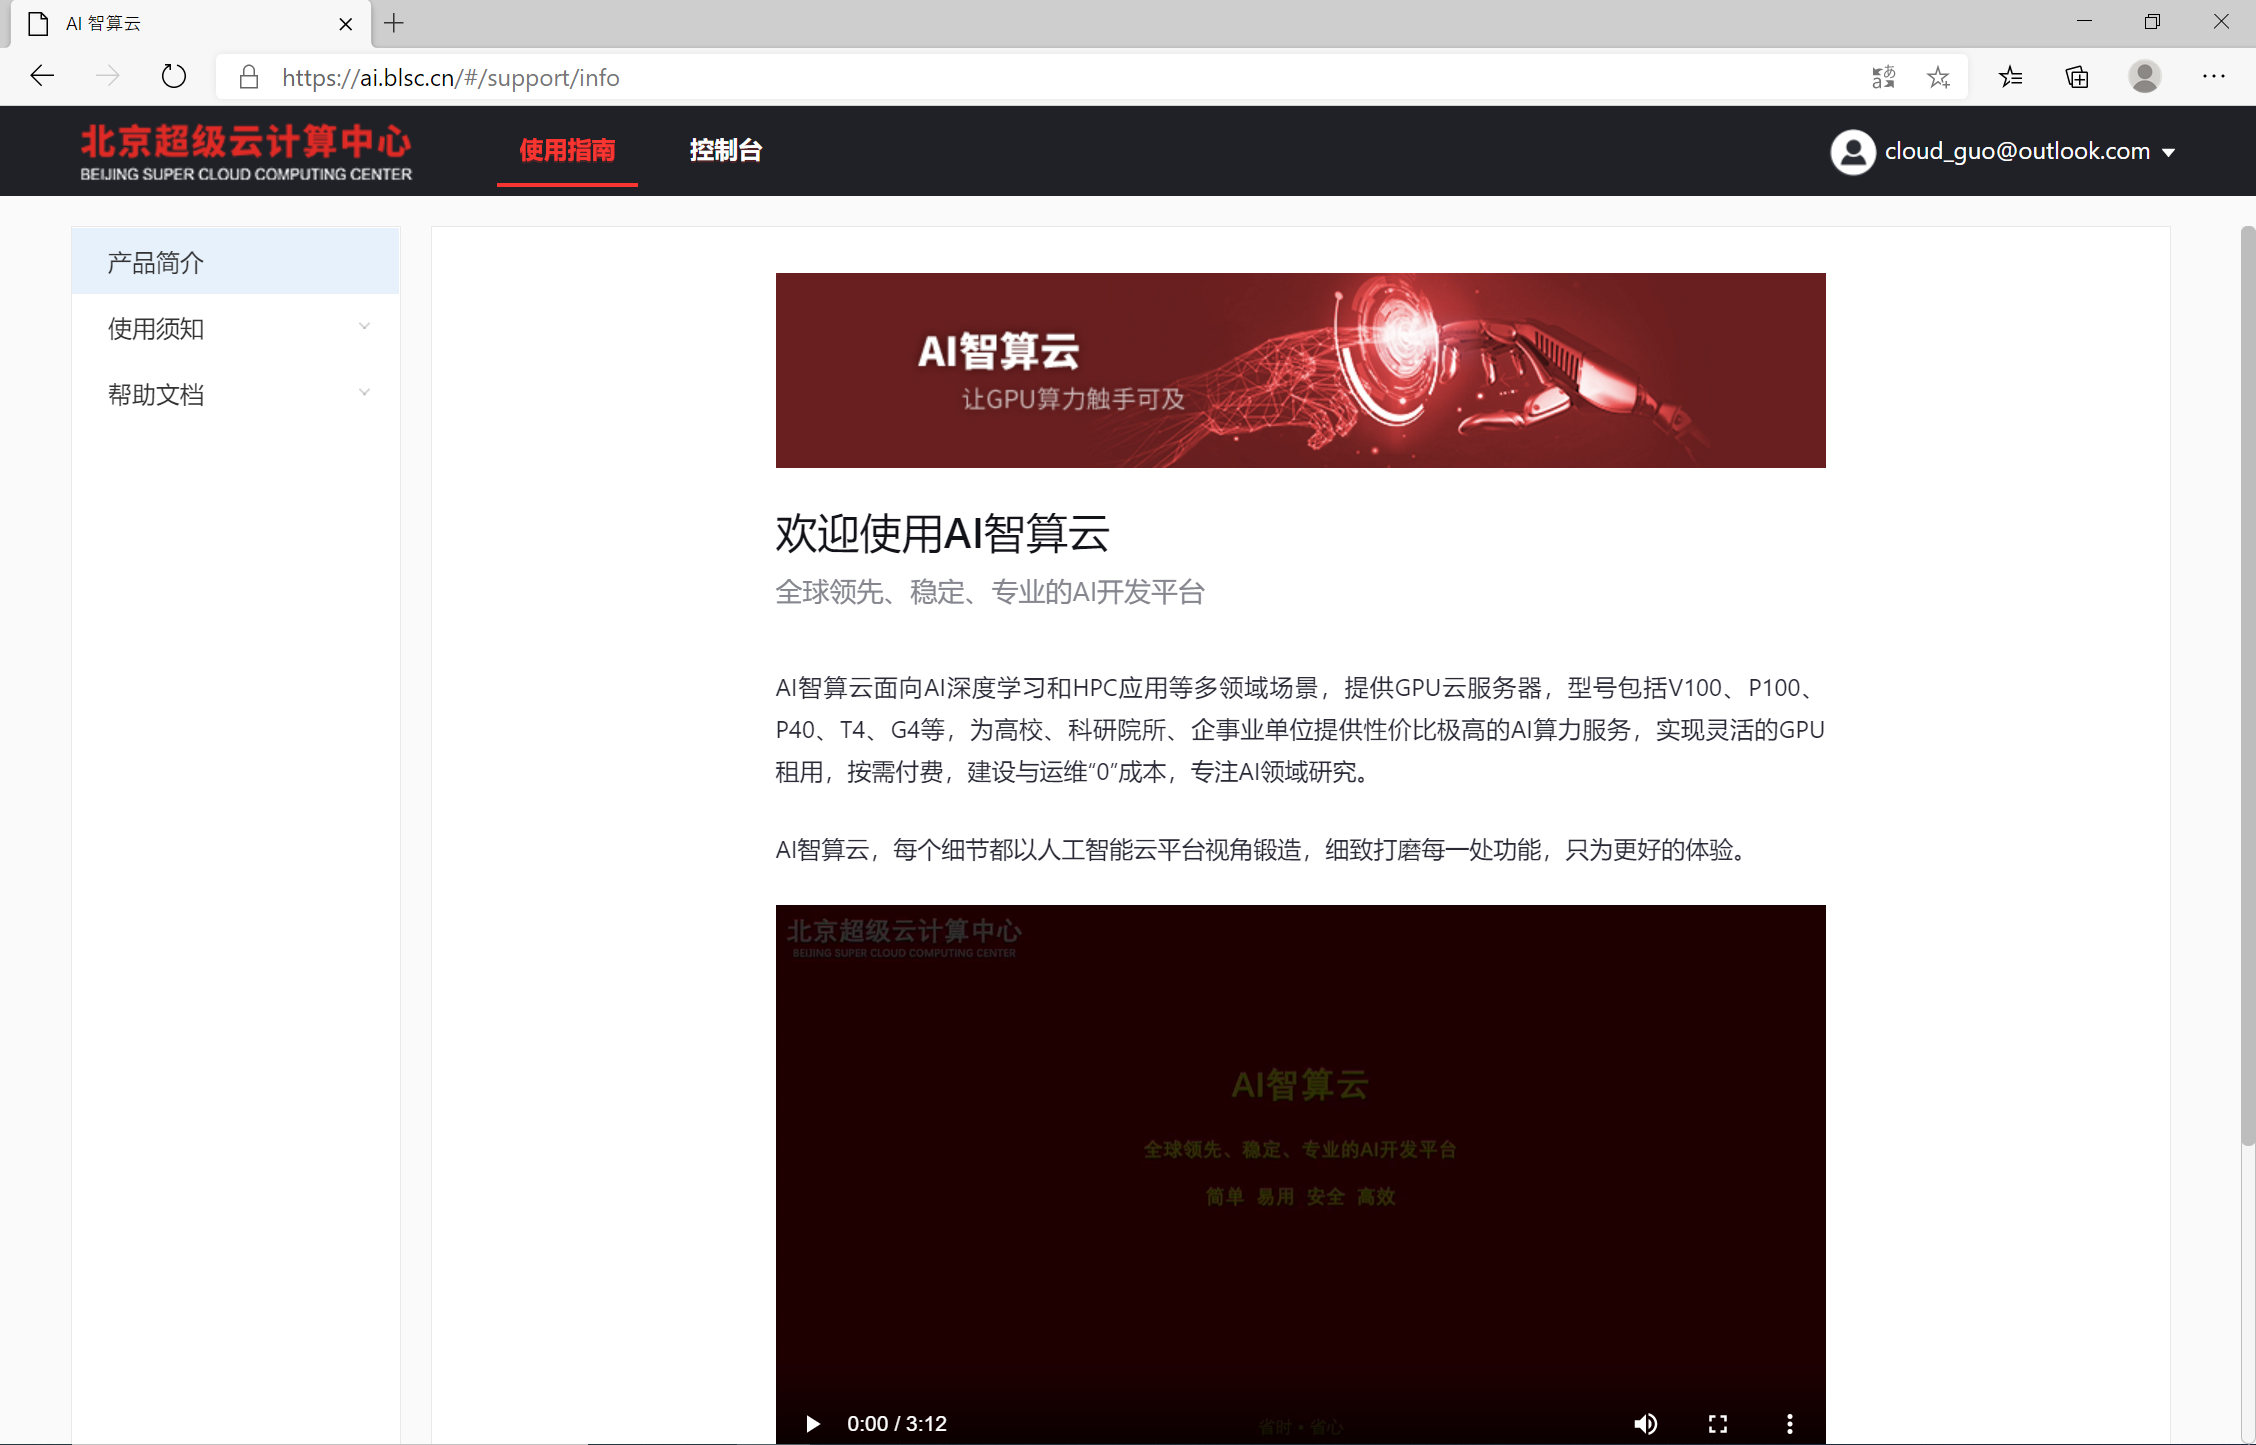
\includegraphics[scale=0.2]{src/img/Welcome.png}
                }

    \end{frame}

    \begin{frame}
        \frametitle{云服务器使用规则}
            \framesubtitle{使用操作流程}

            % \href{https://ai.blsc.cn/#/support/info}{
            %     
\includegraphics{src/img/Tweet.png}
            %     }
            \centering
            \href{https://ai.blsc.cn/\#/support/info}{
                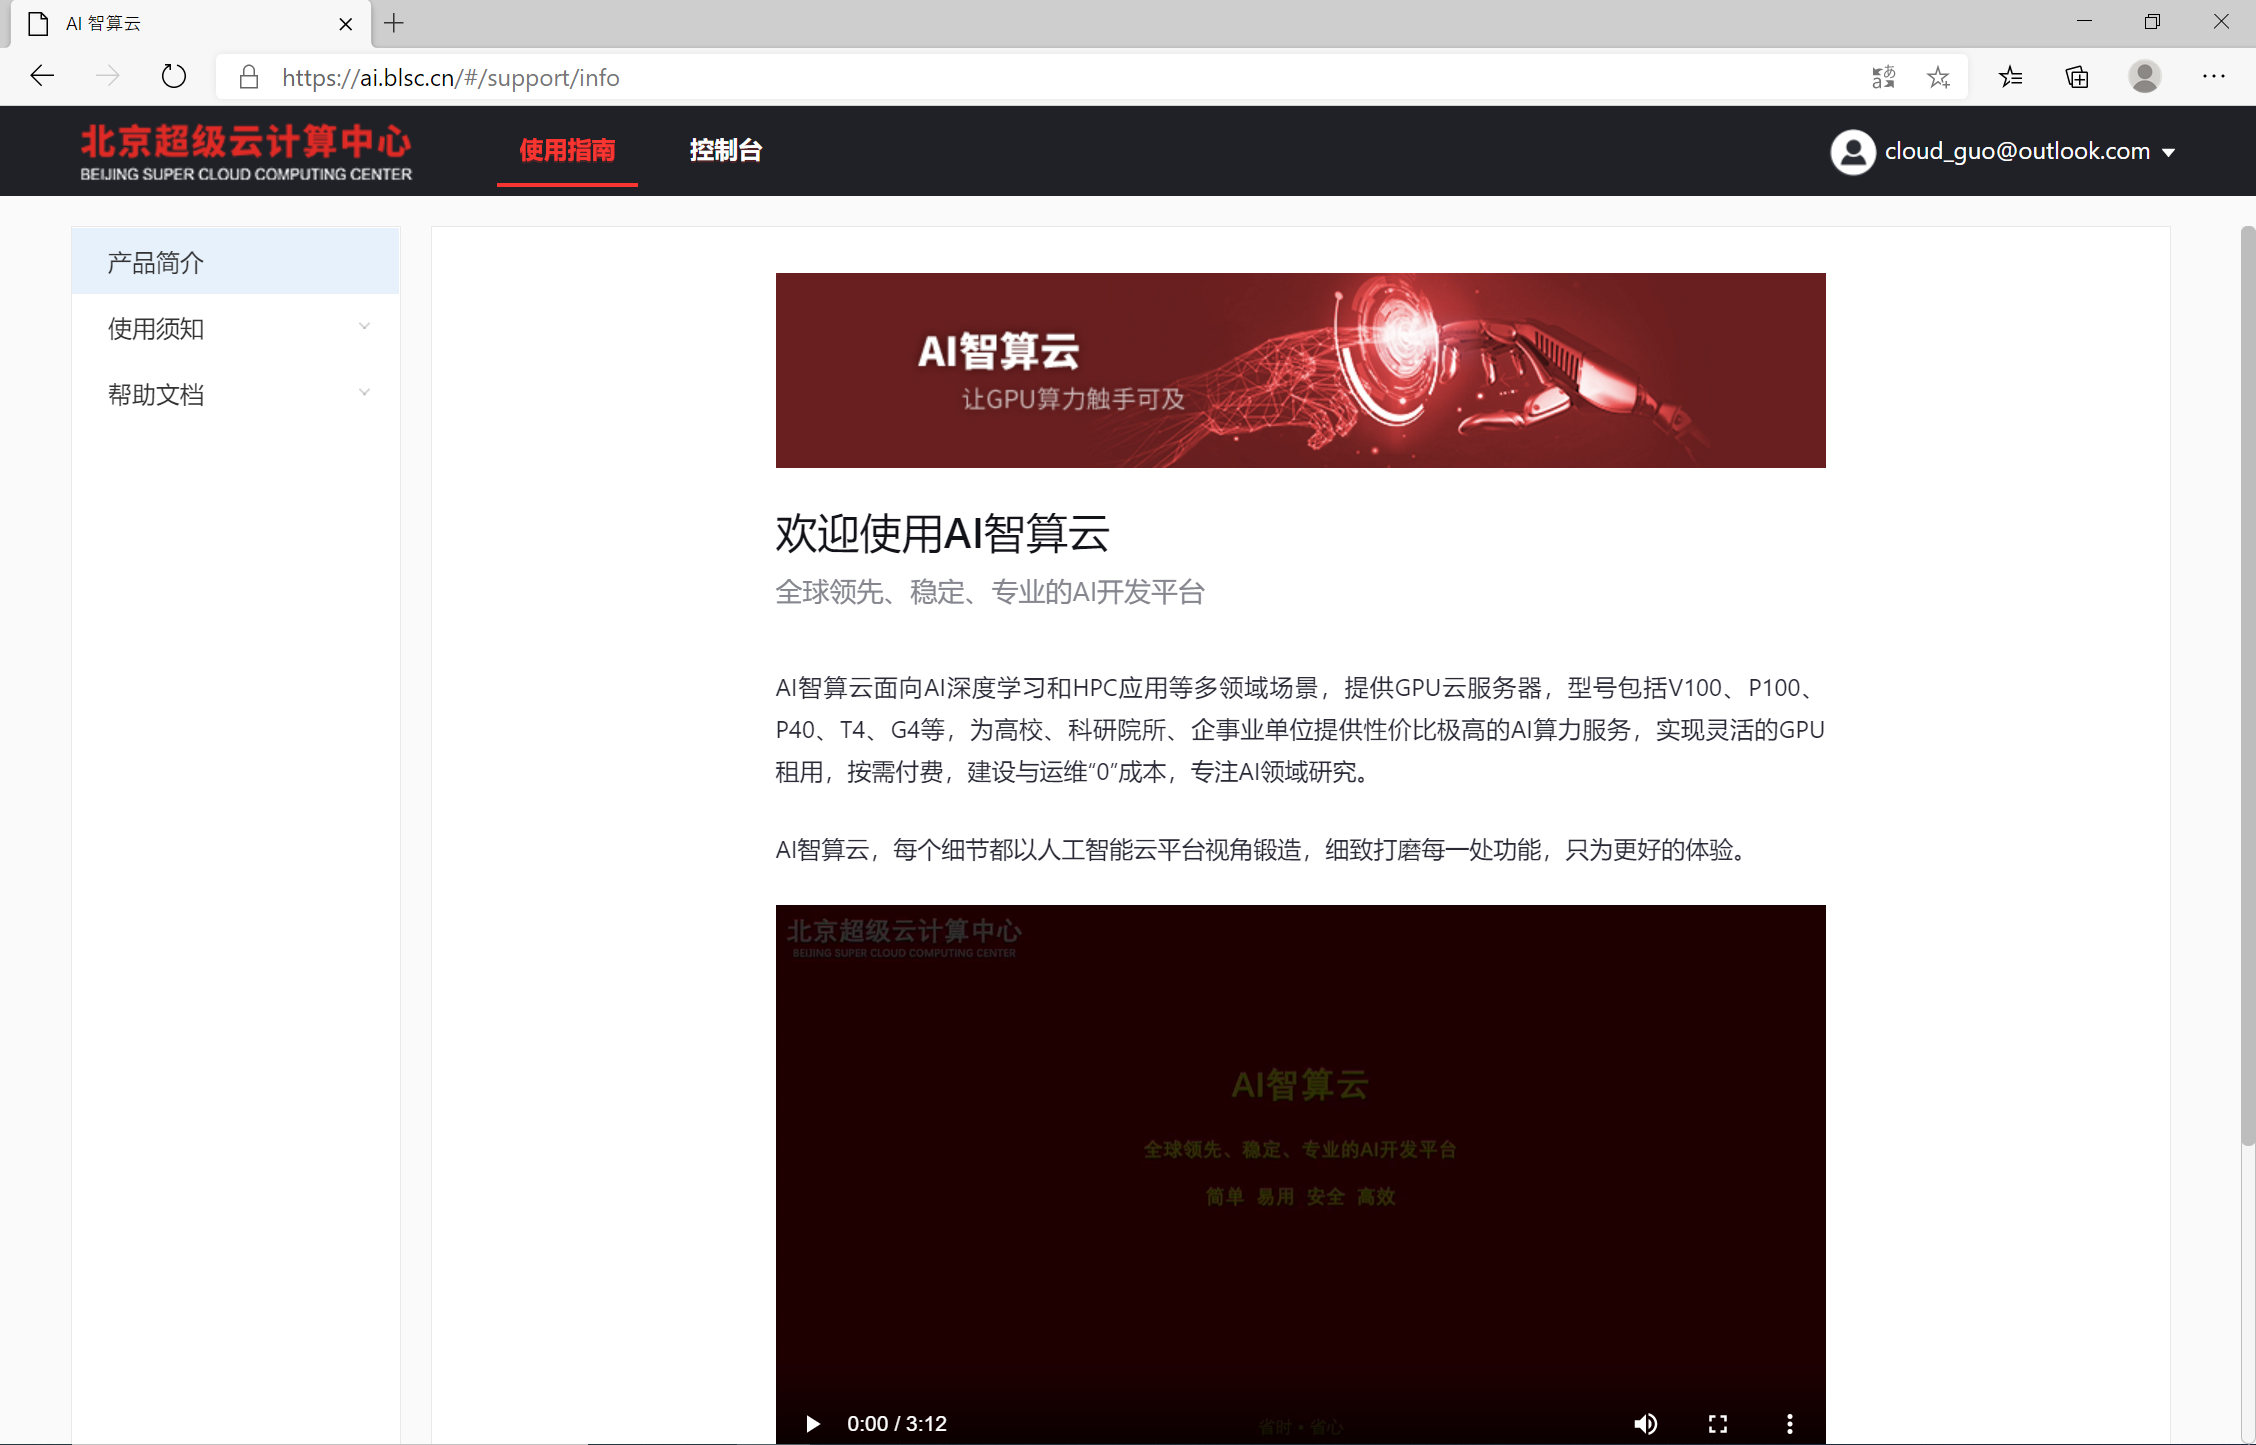
\includegraphics[scale=0.2]{src/img/Welcome.png}
                }

    \end{frame}

\end{document}